\documentclass[12pt]{article}

% Essential Packages
\usepackage{amsmath} % Advanced math typesetting
\usepackage{amsfonts} % Mathematical fonts
\usepackage{amssymb} % Additional mathematical symbols
\usepackage{amsthm} % Theorem formatting
\usepackage{mathtools} % Mathematical tools to improve amsmath
\usepackage{bm} % Bold math symbols
\usepackage{physics} % Simplified physics notations
\usepackage{tikz} % Creating graphics programmatically
\usetikzlibrary{calc,angles,quotes}
\usepackage{pgfplots} % Plotting with LaTeX
\usepackage{wasysym}
\pgfplotsset{compat=newest} % Compatibility setting for pgfplots




% Page and Text Formatting
\usepackage[a4paper,margin=1in]{geometry} % Page size and margins
\usepackage{hyperref} % Hyperlinks
\hypersetup{
    colorlinks=true,
    linkcolor=blue,
    filecolor=magenta,      
    urlcolor=cyan,
}


\title{Methods Notes - Week 6/7}
\author{Kevin Medina \\
        Department of Physics, Florida International University \\
        Course: Mathematical Methods in Theoretical Physics 3113}
\date{\today}




\begin{document}


\maketitle

\section{Introduction}
Complex numbers and functions provide a easier way to represent information making it very useful in physics. A complex number is an ordered pair of two real numbers:

\begin{align*}
	z = (x,y) \\
	z = x+iy
\end{align*}


In General:
\begin{align*}
  (a,b) &\neq (b,a) \\
  (x,y) &\neq (y,x)
\end{align*}

All of complex analysis can be developed in terms of ordered pairs of numbers, variables, and functions:

\begin{equation}
	f(u(x,y),v(x,y))
\end{equation}

\section{Simple Operations}
We can define addition and multiplication opperations for the complex vector space by following a similar form from cartesian space. Addition and multiplication are both defined as:
\begin{equation}
\begin{aligned}
	z_1 \oplus z_2 
	&=(x_1,y_1)+ (x_2,y_2) \\
	&=(x_1+x_2,y_1+y_2)
\end{aligned}
\end{equation}

\begin{equation}
\begin{aligned}
	z_1 \odot z_2 
	&=(x_1, y_1)(x_2,y_2) \\
	&=(x_1 x_2 - y_1 y_2, x_1 y_2 + x_2 y_1) 
\end{aligned}
\end{equation}

Using the definitions above, we can now describe addition and multiplication in the complex space:

\begin{equation}
\begin{aligned}
  (x_1+iy_1)(x_2+iy_2) &= x_1 x_2 + i^2 y_1 y_2 + i(x_1 y_2 + y_1 x_2) \\
  &= (x_1 x_2 - y_1 y_2)+ i(x_1 y_2 + y_1 x_2)
\end{aligned}
\end{equation}

It is convenient to think about a complex number as a vector. Complex numbers, unlike real numbers, do not have cross or dot products. The space of complex numbers is denoted by Z


\subsection{Properties of Complex Numbers}
\begin{enumerate}
\item
Addition or Multiplication of two complex numbers results in a complex number:
\begin{equation}
\begin{aligned}
	z(\oplus , \odot) => z'
\end{aligned}
\end{equation}

\item
	Complex numbers have a zero and unity identity

\item All $z$'s in complex space have an additive and multiplicative inverse:
\begin{equation}
    \begin{aligned}
        \text{Additive Inverse: } & -z \\
        \text{Multiplicative Inverse: } & z^{-1} \text{ or } \frac{1}{z}
    \end{aligned}
\end{equation}

\item If u \& v are complex numbers then $u^v$ is also a complex number.
\end{enumerate}

\subsection{Complex Conjugation}
The division between two vectors is undefined and the same is true for complex numbers. We can resolve this issue by using the complex conjugate of $z$, which is simply the inverse of z.

\begin{equation}
    \begin{aligned}
	    z^* &= x-iy\\
	    z^* &= re^{-i \theta}
    \end{aligned}
\end{equation}

The product of $z$ and $z^*$ results in a real number:
\begin{equation}
    \begin{aligned}
	    z z^* &= (x+iy)(x-iy)\\
		  &= x^2 + y^2\\
		  &= |z|^2  
    \end{aligned}
\end{equation}

Now we can resolve divison of two complex numbers(vectors):
\begin{equation}
    \begin{aligned}
	    \frac{z_1}{z_2} &=\frac{z_1 z_2^*}{z_2 z_2^*}
			    &=\frac{z_1 z_2^*}{|z_2|^2}
    \end{aligned}
\end{equation}

\subsection{Simple Review of \textit{i}}
The imaginary unit, $i$, is simply $\sqrt{-1}$. For reference:
\begin{equation}
    \begin{aligned}
	    i &= \sqrt{-1}\\
	    i^2 &= -1\\
	    i^3 &= -i\\
	    i^4 &= 1
    \end{aligned}
\end{equation}



\section{Representing Complex Numbers in Polar}
A complex number $z$ is often represented in polar form, where:
\begin{equation}
    \begin{aligned}
	    x &= r\cos{\theta}\\
	    y &= r\sin{\theta} \\
	    z &= x + iy \\
	    z &= r(\cos{\theta} + i\sin{\theta})\\
	    z &= re^{i\theta}
    \end{aligned}
\end{equation}

The module of complex number, $z$, is $|z|$ which is equivalent to $r$, they are used interchangeably ($|z| \equiv r$). The module of $e^{i \theta}$ is $1$. We have expressed z in two forms. In terms of cosine and sine, and in Euler's form ($ re^{i\theta}$).Euler's Form is convenient for performing exponential, division, or root operations. Here are a few examples:
\begin{enumerate}
	\item
\begin{equation}
    \begin{aligned}
	    z^n &= (re^{i\theta})^n\\
		&= r^n e^{in\theta}
    \end{aligned}
\end{equation}

\item
\begin{equation}
    \begin{aligned}
	    \frac{1}{z} = \frac{e^{-i\theta}}{r}
    \end{aligned}
\end{equation}

\item
\begin{equation}
    \begin{aligned}
	z_1 &= r_1 e^{i\theta_1}\\
	z_2 &= r_2 e^{i\theta_2}\\
	\frac{z_1}{z_2}&=\frac{r_1}{r_2} e^{i(\theta_1 - \theta_2)}
    \end{aligned}
\end{equation}
\end{enumerate}

\subsection{Euler's Identity}
In addition to representing complex numbers in the polar plane, we also have an important identity to discuss -- Euler's identity:
\begin{equation}
    \begin{aligned}
    1+e^{\pm i \pi}
    \end{aligned}
\end{equation}

The importance of Euler's identity lies in its ability to bridge seemingly unrelated mathematical concepts: exponential functions, complex numbers, and trigonometry. It encapsulates the essence of complex exponentiation and demonstrates that complex exponential functions can produce real values.

\subsection{Derivation of Euler's Formula}
\begin{equation}
    \begin{aligned}
	    e^{i \theta} &= \sum_{n=0}^{\infty}{\frac{(i \theta)^n}{n!}}\\
			 &= \sum_{n=even}^{\infty}{\frac{(i \theta)^n}{n!}} + \sum_{n=odd}^{\infty}{\frac{(i \theta)^n}{n!}}\\
	    e^{i \theta} &= \cos(\theta) + i\sin{\theta}
    \end{aligned}
\end{equation}

\subsection{Root Operations}
Attempting to express $z^{\frac{1}{n}}$, where $n$ is a positive integer, is difficult because of Euler's form. Given, $z^{\frac{1}{n}} = r^{\frac{1}{n}}e^{i(\theta +2k \pi)}$, realise that for any n value, differing choices of k will lead to n distinct values of $z^{\frac{1}{n}}$. All the roots, when sketched on the complex plane, will line up on a circle with radius $r^{\frac{1}{n}}$, and each root would be separated from one another by an angle of $\frac{2\pi}{n}$.

\subsection{On a Circle in Complex}
Following from the previous discussion, becoming familiar with circles in the complex plane is useful for solving counture integrals. In complex a circle is defined as: 

\begin{equation}
    \begin{aligned}
	    |z-z_0| = r
    \end{aligned}
\end{equation}

Where $z_0$ is the center of the circle and $r$ the radius. From this, we can define every point along the circle as:
\begin{equation}
    \begin{aligned}
	    |z-z_0| = re^{i \theta}
    \end{aligned}
\end{equation}
Where $\theta$ is from $0$ to $2\pi$.The differential of this definition of $z$ is $dz = rie^{i \theta}$, where r is constant. This is useful for contour integrals involving a circle/arc/semicircle.  

Example:
\\\textbf{Sketch $z-z_0 = e^{i \theta}$, $\theta \in [0,2\pi)$ on the complex plane and fill in the blank:} 
\\$z-z_0 = e^{i \theta}$ represents a \textit{circle} on the complex plane, which has the \textit{$r=1$} and \textit{$z_0$} at the origin.

\section{Complex Analysis}
\subsection{Analytic Functions}
If $f(z)$ is differentiable and single-valued in a region of the complex plane, it is said to be an \textbf{analytic} function in that region. In order for a complex function, $f(z)$, to be differentiable it must satisfy the \textbf{Cauchy-Riemann} conditions. The conditions are necessary for the existence of a derivative of $f(z)$, thus, in order for $\frac{df}{dz}$ to exist, the \textbf{Cauchy-Riemann} conditions must hold. Simply, we need to guarantee the independance of directionality for the existance of the derivative. Below provides this: 
\begin{align}
	\frac{\delta f}{\delta z} &= \frac{\partial u}{\partial x} + i \frac{\partial v}{\partial x}\\
    \frac{\partial u}{\partial x} &= \frac{\partial v}{\partial y}, \\
    \frac{\partial u}{\partial y} &= -\frac{\partial v}{\partial x},
\end{align}
where $f(z) = u(x, y) + iv(x, y)$, and $z = x + iy$.

\subsubsection*{Example}
Given:$f(z) = u(x,y) + iv(x,y)$, and $u(x,y) = x^2 - y^2$\\
Find:$f(z)$\\
\begin{equation*}
	\pdv{u}{x} = \pdv{(x^2 - y^2)}{x} = 2x
\end{equation*}
\begin{equation*}
	\pdv{u}{y} = \pdv{(x^2 - y^2)}{y}= -2y
\end{equation*}
\begin{equation*}
\int(\pdv{v}{x} = -\pdv{u}{y})dx = \int(2y)dx = 2xy + f_1(y)
\end{equation*}
\begin{equation*}
    v(x,y)=\int(\pdv{v}{y}=\pdv{u}{x})=\int(2x)dy = 2xy + f_2(x)
\end{equation*}

From this $f_1(y) = f_2(x) = C$, $\therefore$
\begin{equation*}
   f(z)=u+iv = x^2 - y^2 + i(2xy+C) = z^2 +iC 
\end{equation*}

\subsubsection*{Remarks}
Recognize that $z^2 = x^2 - y^2 + i(2xy)$\\
This should hold for any form $f(z)$ assumes, even if in the final expression there is no $x$ nor $y$.


\subsection{Singularity and Poles}
A \textbf{singularity} is a function whose values increase towards infinity. A \textbf{pole} is an isolated singularity(a point). Given a fucntion, $f(z)$, then $z_0$ is identified as a pole of order $n$:
\begin{equation}
	f(z) = \frac{g(z)}{(z-z_0)^n}
\end{equation}
\subsubsection{Possible Cases}
\begin{enumerate}
	\item If $n=1$, then $z_0$ is considered to be a \textbf{simple pole}.
	\item $z$ will tend toward infinity as it approaches $0$, this is known as an \textbf{essential singularity}. 
\end{enumerate}

\subsubsection*{Remarks}
The notion of poles and sigularities play an important role in the concepts of residues and various integral theorems including the residue theorem. For the case of a simple pole, a residue is simply the remainder of $f(z)$ after removing the pole. In the simple case of simple poles the remainder is $g(z_0)$


\subsection{Contour Integrals on Complex Planes and Integral Theorems}
Contour integrals, like path integrals, depend on the paths and the end points. We can always calculate the integral of $f(z)$ by noting:
\begin{equation}
    f(z) \equiv u(x,y) +i(x,y)
\end{equation}
\begin{equation}
   dz = d(x+iy) = dx + idy 
\end{equation}
\begin{equation}
	\int_{z_{1}}^{z_{2}}f(z)dz = \int_{z_{1}}^{z_{2}}(u(x+iy)+i(x,y))(dx+idy)
\end{equation}
\begin{equation}
    \int_{z_{1}}^{z_{2}}f(z)dz=\int_{z_{1}}^{z_{2}}(udx-vdy)dx+i \int_{z_{1}}^{z_{2}}(vdx+udy)dy
\end{equation}

Depending on the contour/line/path that is being integrated along and its direction, the $x$ and $y$ are dependent on each other defined by the curve equation.
It could then be simpler to adopt the polar form to calculate contour integrals, especially if it's on a circle. I $z = re^{i\theta}$, then $dz = e^{i\theta}(dr+idr\theta)$,then:
\begin{equation}
    \int_{z_{1}}^{z_{2}}f(z)dz=\int_{z_{1}}^{z_{2}}f(r,\theta)e^{i\theta}(dr+ird\theta)
\end{equation}

On a circle, this integral becomes much simpler, since $r$ is constant, then it would simply become:
\begin{equation}
    \int_{z_{1}}^{z_{2}}f(z)dz=\int_{z_{1}}^{z_{2}}f(r,\theta)e^{i\theta}ird\theta
\end{equation}

\subsubsection{Example - Circle Centered at the Origin}
Integrate $f(z)=z^{n}$ around a circle with a radius $r$ and centered around the origin. 

\begin{enumerate}
	\item Recognize that polar form should be used.
		\begin{equation*}
		    z=re^{i\theta}
		\end{equation*}
		\begin{equation*}
			dz=ire^{i\theta}
		\end{equation*}	
		\begin{equation*}
		    	d\theta \equiv izd\theta
		\end{equation*}
	
	\item Solve the path integral
		\begin{equation*}
			\oint f(z)dz = \oint (re^{i\theta})^n ire^{i\theta} d\theta = \oint (re^{i\theta})^n ire^{i\theta}d\theta = ir^{n+1}\oint e^{i(n+1)\theta}d\theta
		\end{equation*}	

	\item $f(z) = z^{n}$, then 
		    \[ \oint f(z)dz = \begin{cases} 
          0, & n \neq -1 \\
          2\pi i & n = -1 \\
       \end{cases}
    \]
\end{enumerate}

\subsubsection{Example: Integral Over the Rectangular Contour}
Perform the integral of $\oint z^{n}dz$ over the rectangular contour
\begin{equation*}
\mathcal{Z}_1(a-bi) \rightarrow \mathcal{Z}_2(a+bi) \rightarrow \mathcal{Z}_3(-a+bi) \rightarrow \mathcal{Z}_4(-a-bi) \rightarrow \mathcal{Z}_1
\end{equation*}

\begin{enumerate}
	\item Define the paths along each segment. 
	\item Solve the integral for each path, then add all segments together.
\end{enumerate}

\section{Integral Theorems}
Function are required to be analytic in order to apply several integral theorems.
\subsection{Cauchy's first integral theorem}
Cauchy's integral theorem states that: \textit{If $f(z)$ is an analytic function at all points of a simply connected region in the complex plane and if C is a closed contour within that region, then}
\begin{equation}
    \oint_C f(z)dz=0
\end{equation}
A region is \textbf{simply connected} if every closed curve within it can be shrunk continuously to a point that is within the region - A connected region with no holes. The $C$ represents a contour that integrating over. The contour must be "within" the region of analyticity. The integral is path independent. This is crucial for integrals that are difficult to solve due to a complicated path. We can choose a simpler path between two points to solve the same integral.

\subsection{Cauchy's Second Integral Theorem}
Cauchy's Integral formula has remarkable results. The value of an analytic function $f(z)$ is given at an arbitrary interior point $z=z_{0}$ once the values on the boundary $C$ are specified. It must be emphasized that $z_{0}$ is an interior point. The integration along contour is defined in the counter clockwise direction ($CCW$). Here is the integral formula:
\begin{equation}
    \oint \frac{f(z)}{z-z_{0}}dz = 2\pi if(z_{0})
\end{equation}
We can easily observe that there is a pole in our equation. This is of no worry since we can carve out a contour that bypasses this pole. Thus, allowing us to create a new contour based on the original one with an infinitely small opening. This contour will carve out the pole by following a small circular path around the pole. And, again, in a similar manner to the previous theorem, we define the paths along each segment, then, solve the integral for each path, and, finally, add all the segments together.

This theorem has exteions to derivatives. It can be proven using the second integral theorem when $n=0$ and then extend to $n > 1$.
\begin{equation}
    \oint \frac{f(z)}{(z-z_{0})^{n+1}}dz = 2\pi i \frac{f^{n}(z_{0})}{n!}
\end{equation}

In addition, Cauchy's inequality simply states that the product of magnitudes is greater than magnitude of the products.
\begin{equation}
	|f^{n}(z_{0})| = |\frac{n!}{2\pi i} \oint \frac{f(z)}{(z-z_{0})^{n+1}}dz| \leq |\frac{n!}{2\pi i}| \oint \frac{|f(z)|}{|(z-z_{0})^{n+1}|}|dz| 
\end{equation}
\begin{equation}
    =\frac{n!}{2\pi} \frac{f_{max}}{r^{n+1}} (2\pi r) = \frac{n!}{r^{n}}f_{max}
\end{equation}

Recall this to solve the above:
\begin{equation}
    |e^{i(n+1)\theta}|=1
\end{equation}
\begin{equation}
    \oint|dz| = 2\pi r
\end{equation}

The inequality is useful when calculating contour integrals involving infinite circles/semicircles.

\subsection{Residue Theorem}
A powerful theorem that allows us to transform a complicated contour integral intomore manageable algebraic equations. We can use this theorem to derive previously mentioned integral theorems. Residues are what remains after removing a pole from a function. In the case of a simple pole it was simply the function that remained after multiplying by $(z-z_{0})$. For higher pole ordered functions, we must alter our notion to account for the $k^{th}$ order pole at $z_{0}$. This is done by introducing the \textbf{Laurent series}.
\begin{equation}
	f(z) = \frac{h(z)}{(z-z_{0})^{k}} = \sum_{n=0}^{\infty } \frac{h^{m+k}(z)|_{z=z_{0}}}{(m+k)!}
\end{equation}

\begin{equation}
	b_{m} = \frac{h^{m+k}(z)|_{z=z_{0}}}{(m+k)!}
\end{equation}

From this, we find that the residue corrisponds to $b_{-1}$, the coefficient of this Laurent series for the $(z-z_{0})^{-1}$ term. Remember that $m=n-k$.
\begin{equation}
	Residue = R = b_{-1} = \frac{1}{(k-1)!} \frac{d^{k-1}(f(z)(z-z_{0})^{k})}{dz^{k-1}}|_{z=z_{0}}
\end{equation}

In general, we may take various $j-th$ poles, where $0\leq J \leq \infty$, as the integrals along a contour. Each pole contributing to a small circle of $2\pi i R_{j}$ to the total integral.
\begin{equation}
    \oint f(z)dz = \sum_{j} 2\pi i R_{j}
\end{equation}


\subsubsection{Understanding Jordan's Lemma}
Jordan's Lemma is a result in complex analysis that plays a crucial role in evaluating certain types of integrals, particularly when applying the Residue Theorem to compute contour integrals over semi-infinite contours in the complex plane. It is especially useful for integrals involving oscillatory functions, where the path of integration can be closed in the upper or lower half-plane to apply the Residue Theorem effectively.

The lemma states that for a contour \(C_R\) described as a semicircle of radius \(R\) centered at the origin in the upper half of the complex plane, and for a function \(f(z) = e^{iaz}g(z)\), where \(a > 0\) is a real number and \(g(z)\) is a function that is analytic and decreases sufficiently fast as \(|z| \rightarrow \infty\), the integral of \(f(z)\) over \(C_R\) vanishes as \(R \rightarrow \infty\).

Formally, if \(g(z)\) meets the condition that \(|g(z)| \leq \frac{M}{R^n}\) for some \(M > 0\) and \(n > 0\), as \(R \rightarrow \infty\), then:
\[
\lim_{R \rightarrow \infty} \int_{C_R} e^{iaz}g(z) \, dz = 0
\]

\textbf{Application:}
Jordan's Lemma is instrumental in simplifying the computation of integrals by allowing for the evaluation of residues at poles within the contour, while ensuring that the contributions from the semicircular paths at infinity are negligible 


\subsubsection{Using the Residue Theorem to Determine Various Integrals and Apply Jordan's Lemma}
The Residue Theorem is an invaluable tool for computing integrals of real functions that are challenging by traditional means, simplifying these tasks into more manageable algebraic operations. Employing the Residue Theorem typically involves the following essential steps:

\begin{enumerate}
    \item \textbf{Extension to the Complex Plane:} Real functions are extended to the complex plane by replacing the real variable, such as \(x\), with a complex variable \(z\). This step is foundational in applying complex analysis techniques to real integrals.
    
    \item \textbf{Contour Construction:} A closed contour path is constructed in the complex plane. This path may encompass real and/or imaginary axes and is selected so that the complex integrals computed along it are directly related to the original real integrals. To complete the contour, an imaginary path, like semicircles with an infinite radius, is added. 
    
    \item \textbf{Evaluation of Contour Integrals:} The integral over the constructed contour is considered as a sum of integrals over individual paths. By choosing contours wisely—taking advantage of properties like Jordan's Lemma and Cauchy's Inequality—it's often possible to negate the contribution from certain paths, such as those over infinite semicircles (\(R \rightarrow \infty\)).
    
    \item \textbf{Navigating Poles:} When encountering poles within the contour, additional paths may be necessary to avoid singularities. These are usually small circles or semicircles (\(r \rightarrow 0\)) around each pole. The integrals over these small paths can typically be evaluated with ease by expressing \(z\) in polar coordinates, drawing on the principles behind the Residue Theorem itself.
    
    \item \textbf{Application of the Residue Theorem:} Finally, the sum of the path integrals is calculated using the Residue Theorem. This step often reduces to straightforward algebraic computations, thanks to the theorem's ability to simplify the evaluation of complex contour integrals into residues at poles within the contour.
\end{enumerate}



\section{Applications through Problems}
We will show the usage of the concepts by the solutions provied for each complex homework provided.

\subsection{Complex Homework - A}
\begin{enumerate}

	\item Lightening Knowledge Refresher
		\begin{enumerate}

		\item The module($|z| = r$) of $e^{i0.123456788}$ is \_\_?
			\begin{equation*}
				    |e^{i0.123456788}| = 1
			\end{equation*}
		\item Find the values of: $sin(30)$, $cos(45)$, $tan(120)$ - exact answers only.
		\begin{equation*}
			sin(30^{\circ}) = 1
		\end{equation*}	

		\begin{equation*}
			cos(45^{\circ}) = \frac{\sqrt{2}}{2}	
		\end{equation*}	

		\begin{equation*}
			tan(120^{\circ}) = \sqrt{3}
		\end{equation*}	


		\item Sketch a triangle with three sides lengths of 3, 4, and 5 respectively. Note all angles are to be represented as integers approximations. 
			
		\item Sketch a complex plane - $z=x+iy=re^{i\theta}$, and $z^{*}a$, $z^{2}$, $z^{\frac{1}{2}}$. All should be sketched on the same plane with all variables noted properly (assume $r > 1$)

\begin{center}
\begin{tikzpicture}
    % Draw axes
    \draw[thin,->] (-2,0) -- (4,0) node[anchor=north west] {$\Re$};
    \draw[thin,->] (0,-2) -- (0,4) node[anchor=south east] {$\Im$};
    
    % Define z = x + iy = re^{i\theta}
    \def\r{2.5} % r > 1
    \def\angle{40} % Angle theta
    \pgfmathsetmacro{\x}{\r*cos(\angle)} % Real part of z
    \pgfmathsetmacro{\y}{\r*sin(\angle)} % Imaginary part of z
    
    % Draw z
    \draw[thick,->] (0,0) -- (\x,\y) node[midway,above] {$z$};
    \draw[red,thick,dashed] (\x,0) -- (\x,\y) node[midway,right] {$iy$};
    \draw[red,thick,dashed] (0,\y) -- (\x,\y) node[midway,above] {$x$};
    
    % Draw z conjugate
    \draw[thick,->,blue] (0,0) -- (\x,-\y) node[midway,below] {$z^*$};
    
    % Angle theta
    \draw[thick] (1,0) arc (0:\angle:1) node[midway,right] {$\theta$};
    
    % Draw z^2 and z^(1/2) approximately, for demonstration
    % Assuming r > 1, z^2 will be further out and z^(1/2) closer to the origin
    \pgfmathsetmacro{\rSquared}{\r*\r}
    \pgfmathsetmacro{\rSqrt}{sqrt(\r)}
    \pgfmathsetmacro{\xSquared}{\rSquared*cos(2*\angle)}
    \pgfmathsetmacro{\ySquared}{\rSquared*sin(2*\angle)}
    \pgfmathsetmacro{\xSqrt}{\rSqrt*cos(\angle/2)}
    \pgfmathsetmacro{\ySqrt}{\rSqrt*sin(\angle/2)}
    
    % Draw z^2
    \draw[thick,->,green] (0,0) -- (\xSquared,\ySquared) node[near end,above left] {$z^2$};
    
    % Draw z^(1/2)
    \draw[thick,->,purple] (0,0) -- (\xSqrt,\ySqrt) node[near end,below right] {$z^{1/2}$};
    
    % Labels
    \node at (\x/2,-0.3) {$r$};
\end{tikzpicture}
\end{center}
		
		\end{enumerate}


	\item 
		\begin{enumerate}

		    	\item Given $z=3+4i$. Determine the polar form of $z$, $z^{*}$, $\frac{1}{z}$, and $z^{n}$.  Both $a$ and $b$ are real constants. 

			\item Given $z=a+ib$. Determine the polar form of $z$, $z^{*}$, $\frac{1}{z}$, and $z^{n}$.  Both $a$ and $b$ are real constants. 	

		\item $z = \frac{1}{\sqrt{2}} + \frac{1}{{\sqrt{2}}}i$. Determine ($\frac{1}{z^{*}}$) in polar forms and sketch your results in the complex plane. Describe how these results are arranged on the complex plane in words.
		\end{enumerate}
		
	\item 
		\begin{enumerate}

		    \item $z=1+2i$, compute $\frac{z-2z^{*}}{2z+z^{*}}$ and $z^{\frac{1}{3}}$, the sketch all results on the complex plane.

		\item Sketch, on the complex plane, a circle of radius $R=5$ centered at $z_{0} = 2 +i$. Define this circle using the polar form.


		\item $f(z) = e^{z}$. Is it analytic?

		\end{enumerate}



	\item $f(z)=f(x+iy)=u(x,y)+iv(x,y)$; And it's known that $f(z)$ is analytic.
		\begin{enumerate}

		    \item If $v(x,y) = 3x^{2} y-y^{3}$, determine $u(x,y)$ first, then determine $f(z)$ directly in terms of z (the expression should not include x or y), using Cauchy-Riemann relations. If there is any overall integration constant, set it to be equal to $0$.

		\item For part a) function, along the curved path connecting point $A$ at origin and $B$ at $(1+i)$: $\int_{A}^{B}f(z)dz=$?

		\item Similarly, if $u(x,y) = (xcos(y)-ysin(y))e^{x}$, determine if $v(x,y)$ first then $f(z)$ directly in terms of $z$.
		\end{enumerate}

	\item 
		For $f(z) = z^{n}$, determine the contour integral $\oint f(z)dz$ following the rectangular path $(a,b) -> (-a,b) -> (a,-b) -> (a,b) $ in the complex plane. Both a and b are positive real constants.
		\begin{enumerate}

		    \item Sketch the path on the complex plane first and then define $z$ and $dz$ on each of the four

		\item $\oint f(z)dz=$?

		\end{enumerate}
	
	\item
		Consider two paths: $C1:(0,0) -> (1,0) -> (1,1)$, and $C2: (0,0) -> (0,1) -> (1,1)$ in the ocmplex plane.
		\begin{enumerate}

		    \item 
			    $f(z)=z^{2}$; Determine $\oint f(z)dz$ along $C1$ and $C2$; Are the results the same for both paths?

		\item $f(z)=z^{*}$; Determine $\oint f(z)dz$ along $C1$ and $C2$; Are the results the same for both paths?

		\end{enumerate}

	\item Use Cauchy's integral theorems (and/or the extensions) to compute the following(for any closed contour around $z_{0} = i$).
		\begin{enumerate}

			\item $\oint (z-z_{0})^{n}dz =  
		  \begin{cases} 
          ?, & n \neq -1 \\
          ? & n = -1 \\
  \end{cases} $

  \item $\oint \frac{e^{z}+iz^{2}}{z-z_{0}}dz$
	  \item $\oint \frac{e^{z}+iz^{2}}{(z-z_{0})^{3}}dz$
    

		\end{enumerate}

\end{enumerate}

\subsection{Complex Homework - B}
\begin{enumerate}

    \item Knowledge Refresher:
	    Determain, without a calculator, the modules for the following complex numbers: 
	    \begin{enumerate}

	        \item $e^{ilog(e+\theta)}$
		\item $(e^{i0.123456788 \pi})^{2}$
		\item $e^{iz}$, $z=x+iy$ ($x,y$ are real) 
		\item $(re_{-i \theta})^{n}$, $(n,r,\theta$ are all real and positive $)$

	    \end{enumerate}
	
	\item Consider $f(z) = \frac{e^{iz}}{z}$. Determine $\lim_{r\to0} \int_{-r}^{r}f(z)dz$ along the small semicircle shown below, in counterclockwise direction.
	
	\item $f(z)=\frac{e^{iz}-2}{z}$; Determine $\lim_{r\to0}\int_{A}^{B}f(z)dz$ along the arc indicated:

	\item Consider the real function $f(x)= \frac{x^{2}}{(4+x^{2})^{2}}$ and its extension in to the complex plane.
		\begin{enumerate}

		    \item Determine the poles of $f(z)$ and indicate the order of the poles.
			    \item Sketch an appropriate contour that you want to use to determine $\int_{\infty}^{\infty} \frac{x^{2}}{(4+x^{2})^{2}}dx$ and indicate the locations of the poles. Explain how each part of the contour contribute or does not contribute to the integral, and how they are related to $\int_{\infty}^{\infty} \frac{x^{2}}{(4+x^{2})^{2}}dx$

		\item Determine $\int_{\infty}^{\infty} \frac{{x^{2}}(4+x^{2})^{2}}dx$

		\end{enumerate}

\item Consider the real function $f(x)= \frac{x^{2}}{(1+x^{4})}$ and its extension into the complex plane.
	\begin{enumerate}

	    \item Determine the simple poles of $f(z)$
	\item Use the residue theorem to determine $\int_{\infty}^{\infty} f(x)dx$ using a contour that include the real axis and the upper semicirle with a radius $R \to \infty$
	
	\item Repeat part b), but use a new contour(there is more than one choice) that involves both real and imaginary axes. Your contour cannot have a semicircle.

	\item Repeat part b), but use a different semicircle that only involves that imaginary axis, not the real one.

	\end{enumerate}

	\item Consider the real function $f(x) = \frac{sin^{2}(x)}{x^{2}}$ and its extention into the complex plane. Note $sin^{2}(x) = \frac{1-cos(2x)}{2}$, and replace $cos(2x)$ with $e^{i2z}, x^{2}$ with $z^{2}$
		\begin{enumerate}

		    \item Determine the residue of the double(not simple) pole of f(z) at z=0
		\item Determine $\int_{\infty}^{\infty} f(z)dz$ - Cauchy's integration theorem and residue theorem are needed, and symmetry consideration (Hint: Choose a contour that includes the real axis and the upper semicircle with a radius $R \to \infty$. However, since the pole is on the real axis, you need to come up with another small upper semicircle around the pole to get around it)


		\end{enumerate}


	\item Consider the real function $f(x) = \frac{cos(kx)}{(x^{2}+a^{2})}$ and its extension into the complex plane, by replacing $cos(kx)$ with $e^{ikz}$, $x^{2}$with $z^{2}$. ($k$ and $a$ are positive, real constants) 
		\begin{enumerate}

		    \item Determine the poles of f(z)
		\item Come up with a proper contour so that you could use residue theorem and determine $\int_{\infty}^{\infty} f(x) dx$

		\end{enumerate}

	\item In order to prove Cauchy's first integral theorem, we used Cauchy's condition for analytic complex functions as well as the Stoke's theorem to show that the real part of the integral $\oint f(z)dz=0$. Similarly, show that the imaginary part of $\oint f(z)dz=0$ as well. $f(z) \equiv u(x,y)+iv(x,y)$.

	\item The residue for the function $\frac{1}{x^{4}+1}$ at $z_{1}=e^{\frac{i\pi}{4}} \equiv \frac{\sqrt{2}}{2}(1+i)$; Compute the residues at the other three poles as well.

\end{enumerate}


\newpage
\section{The Unit Circle}
The unit circle and it's corresponding angles are provided in both degree's and radians.
\begin{center}
	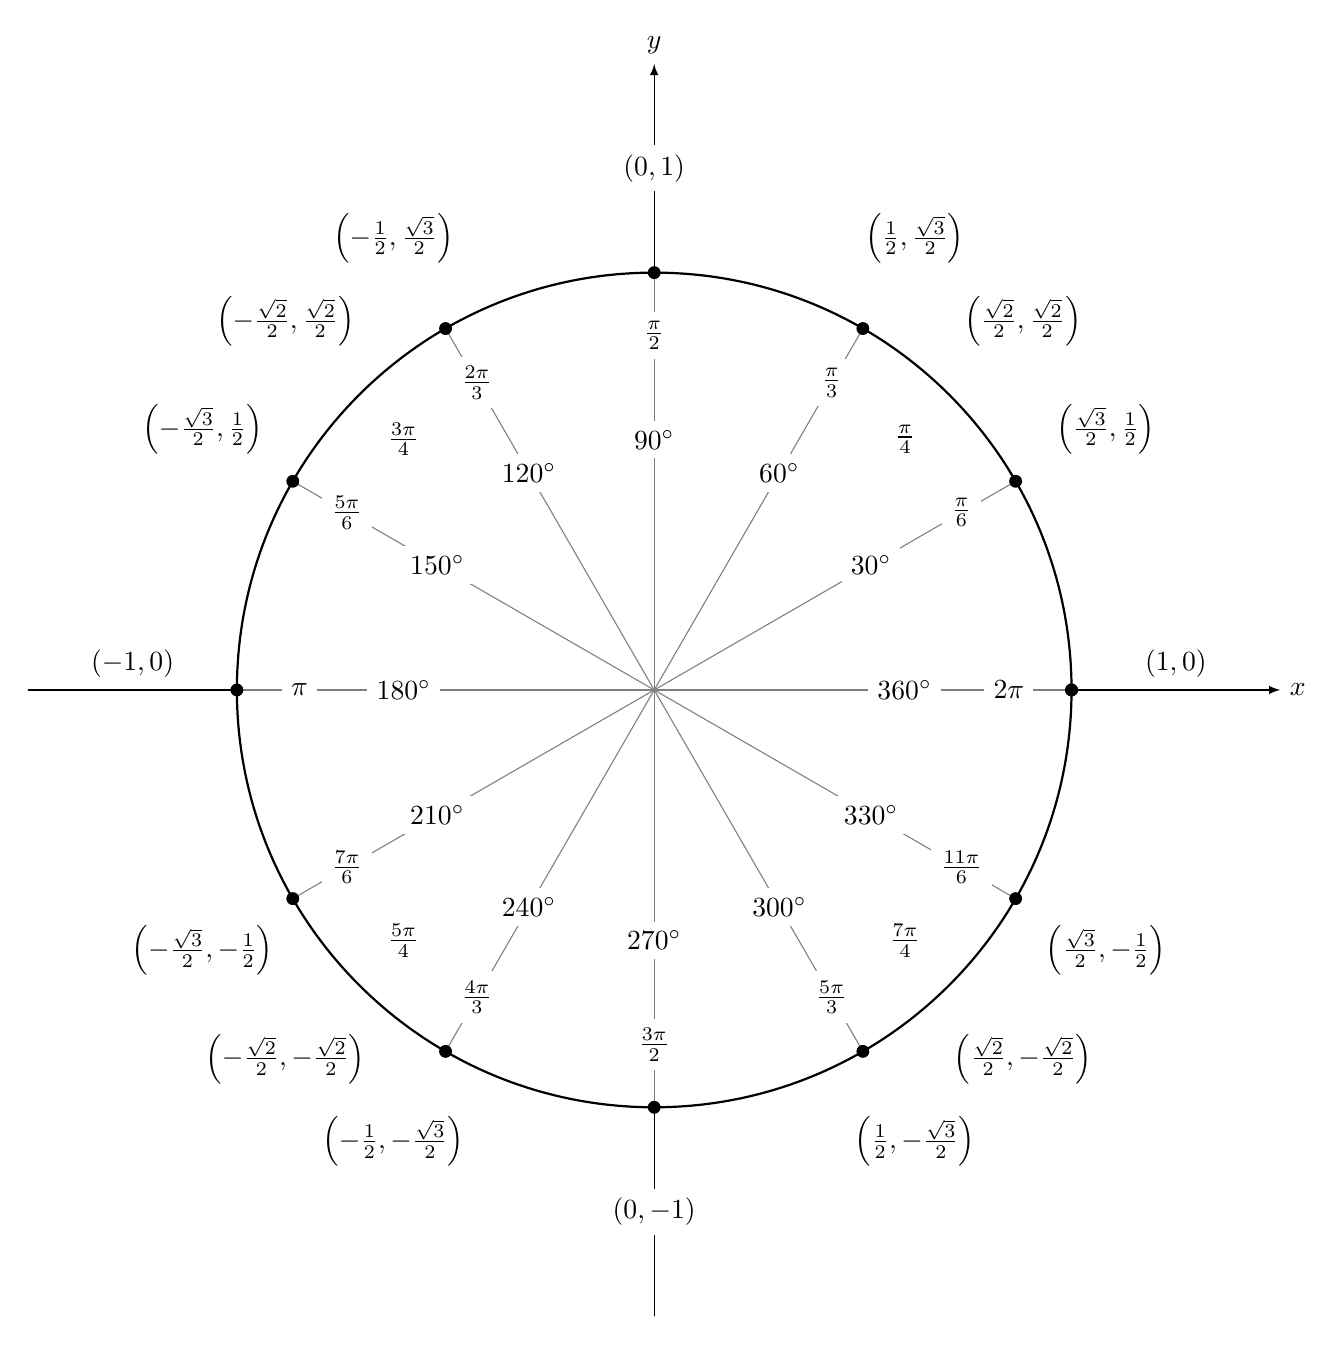
\begin{tikzpicture}[scale=5.3,cap=round,>=latex]
        % draw the coordinates
        \draw[->] (-1.5cm,0cm) -- (1.5cm,0cm) node[right,fill=white] {$x$};
        \draw[->] (0cm,-1.5cm) -- (0cm,1.5cm) node[above,fill=white] {$y$};

        % draw the unit circle
        \draw[thick] (0cm,0cm) circle(1cm);

        \foreach \x in {0,30,...,360} {
                % lines from center to point
                \draw[gray] (0cm,0cm) -- (\x:1cm);
                % dots at each point
                \filldraw[black] (\x:1cm) circle(0.4pt);
                % draw each angle in degrees
                \draw (\x:0.6cm) node[fill=white] {$\x^\circ$};
        }

        % draw each angle in radians
        \foreach \x/\xtext in {
            30/\frac{\pi}{6},
            45/\frac{\pi}{4},
            60/\frac{\pi}{3},
            90/\frac{\pi}{2},
            120/\frac{2\pi}{3},
            135/\frac{3\pi}{4},
            150/\frac{5\pi}{6},
            180/\pi,
            210/\frac{7\pi}{6},
            225/\frac{5\pi}{4},
            240/\frac{4\pi}{3},
            270/\frac{3\pi}{2},
            300/\frac{5\pi}{3},
            315/\frac{7\pi}{4},
            330/\frac{11\pi}{6},
            360/2\pi}
                \draw (\x:0.85cm) node[fill=white] {$\xtext$};

        \foreach \x/\xtext/\y in {
            % the coordinates for the first quadrant
            30/\frac{\sqrt{3}}{2}/\frac{1}{2},
            45/\frac{\sqrt{2}}{2}/\frac{\sqrt{2}}{2},
            60/\frac{1}{2}/\frac{\sqrt{3}}{2},
            % the coordinates for the second quadrant
            150/-\frac{\sqrt{3}}{2}/\frac{1}{2},
            135/-\frac{\sqrt{2}}{2}/\frac{\sqrt{2}}{2},
            120/-\frac{1}{2}/\frac{\sqrt{3}}{2},
            % the coordinates for the third quadrant
            210/-\frac{\sqrt{3}}{2}/-\frac{1}{2},
            225/-\frac{\sqrt{2}}{2}/-\frac{\sqrt{2}}{2},
            240/-\frac{1}{2}/-\frac{\sqrt{3}}{2},
            % the coordinates for the fourth quadrant
            330/\frac{\sqrt{3}}{2}/-\frac{1}{2},
            315/\frac{\sqrt{2}}{2}/-\frac{\sqrt{2}}{2},
            300/\frac{1}{2}/-\frac{\sqrt{3}}{2}}
                \draw (\x:1.25cm) node[fill=white] {$\left(\xtext,\y\right)$};

        % draw the horizontal and vertical coordinates
        % the placement is better this way
        \draw (-1.25cm,0cm) node[above=1pt] {$(-1,0)$}
              (1.25cm,0cm)  node[above=1pt] {$(1,0)$}
              (0cm,-1.25cm) node[fill=white] {$(0,-1)$}
              (0cm,1.25cm)  node[fill=white] {$(0,1)$};
    \end{tikzpicture}
\end{center}


\end{document}
